\documentclass[a4paper,11pt]{article}

\usepackage[T1]{fontenc}	      %font - (base) HA ALLTID MED
\usepackage{lmodern}						%font - Standard
%---
\usepackage[english]{babel}   %svenska
\usepackage[utf8]{inputenc}   %svenska åäö
\usepackage{lipsum}           %onödiga texten
\usepackage{booktabs}         %referat
\usepackage{amsmath, amssymb, upref} %matte
\usepackage{amsthm}           %omgivningar
\usepackage{gensymb}
%---
\usepackage{caption}
\usepackage{subcaption}	%använd antingen cap & subcap ELLER hyperref
%---
\usepackage{tocbibind}        %till referenser i innehållsförteckning
\usepackage{graphicx}         %till implementering av bilder
\usepackage{color}						%för text i färg
\usepackage[framemethod=tikz]{mdframed}	%highlighting hela stycken
\usepackage{listings}	%för kod
\usepackage{lr-cover}         %Roberts förstasida
\usepackage{labrapport}				%Roberts rapportmall

\usepackage{setspace}	%line space
	\singlespacing

\definecolor{dkgreen}{rgb}{0,0.6,0}		%för kod
\definecolor{gray}{rgb}{0.5,0.5,0.5}	%för kod
\definecolor{mauve}{rgb}{0.58,0,0.82}	%för kod

\lstset{	%för kod
	frame=tb,
  language=C,
  aboveskip=3mm,
  belowskip=3mm,
  showstringspaces=false,
  columns=flexible,
  basicstyle={\small\ttfamily},
  numbers=none,
  numberstyle=\tiny\color{gray},
  keywordstyle=\color{blue},
  commentstyle=\color{dkgreen},
  stringstyle=\color{mauve},
  breaklines=true,
  breakatwhitespace=true,
  tabsize=3
}

\newcommand{\highlight}[1]{\colorbox{yellow}{#1}}	%highlighting små stycken

\long\def\*#1*/{}	%kommentarer - \* nu skriver jag en kommentar */

\begin{document}

\title{Project Report - 3D Programming for Master of Science in Engineering}
\author{Filip Pentikäinen}
\date{\today}
\maketitle

\section{Introduction}
In this project a variety of different 3D rendering techniques is implemented. These are:
\begin{enumerate}
	\item \textit{(Core)} Deferred rendering and lighting
	\item \textit{(Geometry)} Parsing and rendering of an existing model format (OBJ)
	\item \textit{(Projection)} Shadow mapping
	\item \textit{(Acceleration)} Back-face culling using geometry shader
	\item \textit{(Other)} Glow-effect using compute shader (bloom)	
\end{enumerate}

This report will mostly focus on the GPU implementation of the techniques and how they affect the final image. This project was implemented using DirectX 11.

\newpage
\section{Deferred rendering and lighting}
Implementing deferred rendering means to divide the basic rendering process into several stages (or \textit{passes}). The first pass is responsible for drawing all objects, and then outputting several textures with information about the scene. These textures hold data for each pixel-hit object regarding the normal, diffuse albedo, specular albedo and world position.

This information is then transferred to the next pass, the \textit{light shading}-pass, where all this data, in combination with information of the different lights in the world, is used to create a scene with \textit{phong} lighting. The phong shading technique is the combination of ambient, diffuse and specular light to create phong reflection (see Figure 1). 

\begin{figure}[ht!]
	\begin{center}
		\label{phong}
		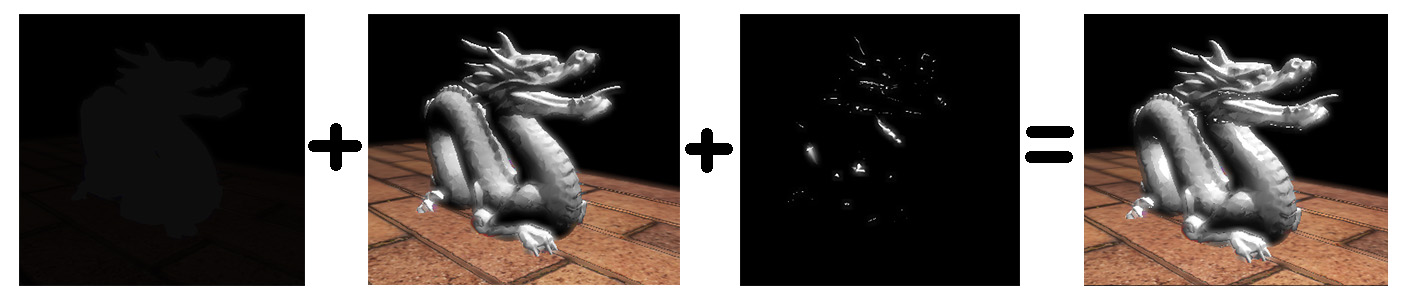
\includegraphics[width=11cm]{pic/comparison2.jpg}
		\caption{ambient + diffuse + specular = phong reflection}
	\end{center}
\end{figure}

The attenuation factor (light weakening with distance) is then added to the final color calculations to finalize the lighting stage. The attenuation is different depending on what kind of light we use. If directional light (the sun) is used, then attenuation does not exist. If the light is a spotlight (torch/flashlight) or a pointlight (lightbulb), then the light fades as the distance to the light becomes greater. Directional light has another attenuation factor, where the light shines less bright the farther from the direction of the light the point is.

\begin{figure}[ht!]
	\begin{center}
		\label{fin}
		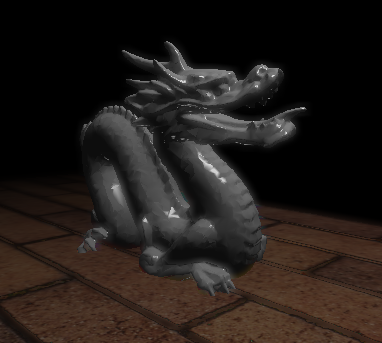
\includegraphics[width=7cm]{pic/fin.png}
		\caption{Final output with phong shading and attenuation}
	\end{center}
\end{figure}

The final color is then drawn on a fullscreen quad and output.

\newpage
\section{Parsing and rendering of an existing model format (OBJ)}
Parsing a model means to read a file containing data about a 3D object. These files contain geometric vertices, texture vertices and vertex normals. The information is later combined to create 3 points in space complete with texture coords and normals, representing a triangle (see Figure 3 and 4).

\begin{figure}[ht!]
\begin{lstlisting}
	mtllib box.mtl
	v -0.500000 -0.500000 0.500000	//point position
	v 0.500000 -0.500000 0.500000
	v -0.500000 0.500000 0.500000
	...
	vt 0.375000 0.000000	//point u-v coords
	vt 0.625000 0.000000
	vt 0.375000 0.250000
	...
	vn 0.000000 0.000000 1.000000	//point normal
	vn 0.000000 0.000000 1.000000
	vn 0.000000 0.000000 1.000000
	...
	f 1/1/1 2/2/2 3/3/3	//using the 1st, 2nd and 3rd row respectivly of the different datapoints to create a triangle
	...
\end{lstlisting}
\caption{Sample of an OBJ file}
\end{figure}

\begin{figure}[ht!]
\begin{lstlisting}
	while (/*...*/){
		int res = fscanf(file, "%s", lineHeader);
		
		if (strcmp(lineHeader, "v") == 0) {
			//save the component into an array
		}
		//...
		else if (strcmp(lineHeader, "f") == 0) {
			fscanf(file, "%i/%i/%i %i/%i/%i %i/%i/%i\n", /*...*/);
			for (short i = 0; i < 3; i++){
				//save the 3 faces 1 by 1 in the array, ready to be handled by the vertex shader
			}
		}
	}
\end{lstlisting}
\caption{C code for parsing OBJ file}
\end{figure}

To parse this information, firstly the data type (v, vt, vn and f) is parsed and identified. Then the data is sorted into arrays accordingly. Once the triangles are being assembled (f), the data is already stored in RAM, and we do not need to access secondary storage. The data is stored in a 1D array where every 3 elements are combined in the vertex shader in the first pass to create a triangle.

An MTL file usually accompanies an OBJ file which contains data related to the material color, illumination, ambient reflectivity, diffuse reflectivity, transmission filter and texture name. These properties are read with the OBJ and later sent to the fragment shader in the first pass to be used in creating the textures for diffuse- and specular albedo.

\newpage
\section{Shadow mapping}
Shadow mapping is the technique of creating shadows through the use of the lights view. The basic concept is that the entire scene is created from the lights point of view and the depth to every point hit by a pixel is saved in a texture, the so-called \textit{shadow map}.

During the light calculations, the depth values saved in the shadow map are compared to the length of the vector between the final pixel points and the light. If the shadow map's depth is lower, that means there is an object in the way, hence the pixel is occluded.

Implementing the shadow pass, where the scene is rendered from the lights point of view, is very simple. We just need to pass the same data to this vertex shader as we did to the original vertex shader but this time we change the view and perspective matrices to the ones belonging to the light. The rasterizer only needs to draw the depth values to a texture, which it does anyway for saving data on what objects are in front of others in the scene, and we save that texture and reuse it in the \textit{light shading}-pass from deferred rendering.

In the \textit{light shading}-pass the pixel points world position (accessed via a texture from the first pass) is then multiplied with the view- and perspective matrices and divided by the \textit{w}-element to get the pixel points position from the light. We then recalculate the 2D position of the space from (-1 to 1) to (0 to 1). After that we sample the shadow map in that 2D location. A small $\epsilon$ is added to the shadow map's depth to prevent shadow acne. Implementation can be seen in Figure 5 and 6. 

\begin{figure}[ht!]
\begin{lstlisting}
	float4 newPos = mul(float4(pixelPos3D, 1.0f), mul(ViewMatrixLight, ProjectionMatrixLight));
	newPos.xyz /= newPos.w;

	float2 textureCoordinates = float2((newPos.x / 2.0) + 0.5, (newPos.y / -2.0) + 0.5);

	float depthValue = ShadowMapTexture.Sample(sampAni, textureCoordinates).r + 0.0001f;

	//return a light strength
	if (depthValue < newPos.z) return 0.0;
	else return 1.0;
\end{lstlisting}
\caption{Function that reads the shadow map in the correct location and returns a brightness factor}
\end{figure}

\begin{figure}[ht!]
	\begin{center}
		\label{fin}
		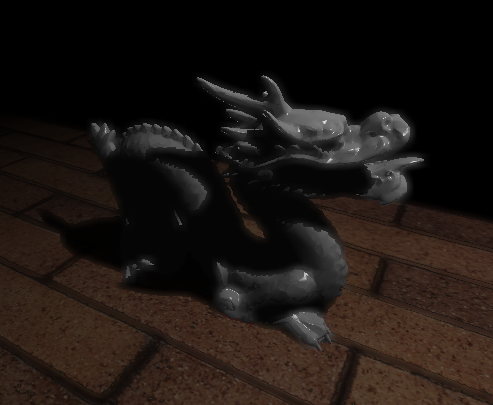
\includegraphics[width=7cm]{pic/final_shadow.png}
		\caption{phong lighting + attenuation + shadow mapping}
	\end{center}
\end{figure}

\newpage
\section{Back-face culling using geometry shader}
Back-face culling is the elimination of triangles facing away from the camera. These triangles would have displayed the backside of the object if shown, which is not desired. It also lightens the load of the first pass where all objects are drawn in 3D.

To determine of the face is not facing the camera, the dot product between the face's normal and a vector from the camera and the hitpoint is calculated. If the angle is greater than $90\degree$ then the triangle is culled. For a visual (and \textbf{very} well drawn) representation, see Figure 7. For source, see Figure 8.

\begin{figure}[ht!]
	\begin{center}
		\label{fin}
		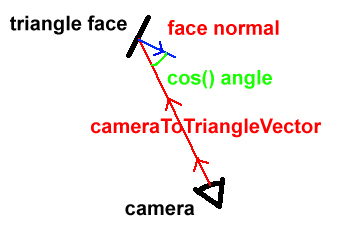
\includegraphics[width=7cm]{pic/backfaceCulling.jpg}
		\caption{Beautiful illustration of backface culling}
	\end{center}
\end{figure}

\begin{figure}[ht!]
\begin{lstlisting}
	//...
	if (/*first point of triangle*/) {
	 float3 cameraToTriangle = (float3)output.PositionWS - CamPos;
	 float dotproduct = dot(cameraToTriangle, output.NormalWS);
	 
	 if (dotproduct > 0.0f) { //cull
	  //discard the triangle
	 }
	}
	//...
\end{lstlisting}
\caption{Determining the angle between the vectors and potentially culling}
\end{figure}

\newpage
\section{Glow-effect using compute shader (bloom)}
A bloom effect is when nearby light overshines/bleeds onto darker areas. This is done in post processing after the light shading pass, once the image is complete. The calculations are done per-texel and are very expensive.

The first step is to gather information of the surrounding texels. This is done by a double for-loop filling a 2D array with colors. These colors are later tested to see if they are brighter than the original texel and, if they are, the screen-space distance between the color-texel and the original texel (creating a fading glow). A new texture is then filled with new colors from the compute shader. See Figure 9 and 10 for demonstration.

\begin{figure}[ht!]
	\begin{center}
		\label{fin}
		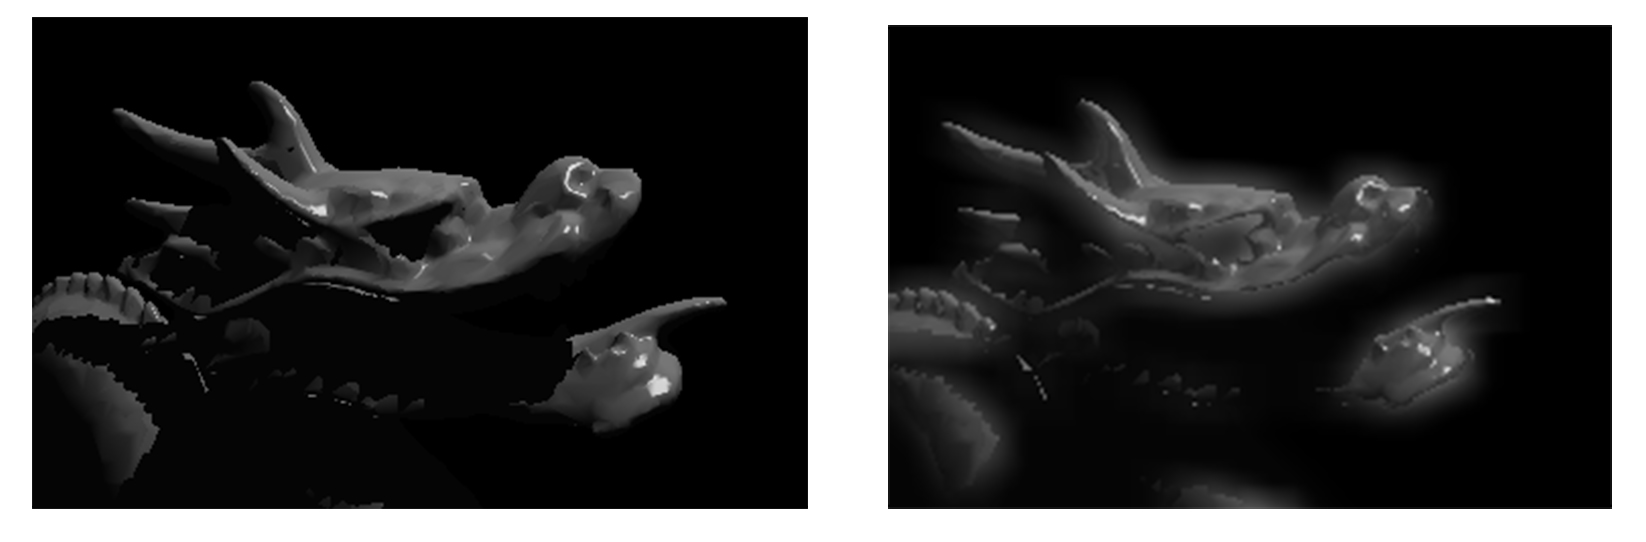
\includegraphics[width=10cm]{pic/glowComparison.jpg}
		\caption{Comparision between output texture with and without bloom. Shot daken from a far distance}
	\end{center}
\end{figure}

\begin{figure}[ht!]
\begin{lstlisting}
	//...
	float4 texelColorArray[RANGE*2][RANGE*2];
	
	for (int x1 = 0; x1 < 2*RANGE; ++x1) {
	 for (int y1 = 0; y1 < 2*RANGE; ++y1) {
	  //save texel data into texelColorArray[][]
	 }
	}
	
	for (int x = 0; x < RANGE*2; ++x) {
	 for (int y = 0; y < RANGE*2; ++y) {
	  float constValues = /*bleedrate, distance & decline*/;
	  if (texelColorArray[x][y].r > (startColor.r * TRIGGERPOINT))
	   finalColor.rgb += (texelColorArray[x][y].rgb * constValues);
	 }
	}
	//...
\end{lstlisting}
\caption{Compute shader for creating bloom-effect}
\end{figure}

\newpage
\begin{thebibliography}{3}

	\bibitem{bok 1}
		 Tomas, Akenine-Möller, Eric, Haines, Naty, Hoffman, \textit{Real-Time Rendering}, 3rd edition, A K Peters Ltd, $2008$.
		
	\bibitem{bok 2}
		 Zink, Jason, Pettineo, Matt, Hoxley, Jack, \textit{Practical Rendering and Computation with Direct3D 11}, 1st edition, $2011$.
		
\end{thebibliography}

\end{document}